\documentclass[a4paper,10pt]{article}
\usepackage[utf8]{inputenc}
\usepackage[polish]{babel}
\usepackage{polski}
\usepackage{graphicx}
\usepackage{hyperref}
\hypersetup{colorlinks,citecolor=black,filecolor=black,linkcolor=black,urlcolor=black,pdftex}

\title{Temat projektu: Przeprowadzanie operacji cyfrowych na~obrazach, za pomocą z~wizualizowanego systemu blokowego.\\Nazwa kodowa: PIWO - Projekt Informatyczny Wilq \& Others.}
\author{Piotr Wilk \and Piotr Zegar \and Mateusz Tylek \and Mateusz Kocąb \and Wojciech Zbiegieł \and Sławomir Librant \and  Marek Prząda}
\begin{document}
\maketitle
\begin{figure}[h]
 \centering
 
\includegraphics{logo}
\begin{center}
\begin{center}

\end{center}

 % logo.eps: 0x0 pixel, 300dpi, 0.00x0.00 cm, bb=0 0 160 154
\end{center}

\end{figure}
\newpage
\tableofcontents
\newpage

\section{Etap wstępny}
\subsection{Opis dziedziny przedmiotowej}
Dziedziną projektu jest grafika, w~głównej mierze operację cyfrowe. 
\subsection{Cel projektu – po co?}
Celem projektu jest zrealizowanie programu umożliwiającego cyfrowe przetwarzanie obrazu, jako z wizualizowanego ciągu bloków, na każdym z nich będzie dodana możliwość poglądu obrazu w~każdym jego stadium przekształcania. Użytkownik będzie mógł dodawać własne typy danych jaki i funkcji operujących na nich. 
\subsection{Zakres projektu – co i jak?}
\begin{enumerate}
\item stworzenie dokumentacji
\item zrealizowanie graficznego interfejsu
\item implementacja operacji przetwarzania obrazu takich jak: \\
(wybór pozostawiony dla pozostałych osób z grupy)
\item dodanie opcji tworzenia własnych dodatków (plug-in)
\end{enumerate}
\subsection{Opracowanie wymagań wstępnych}
\subsubsection{Oczekiwana funkcjonalność systemu}
Możliwość:
\begin{enumerate}
 \item tworzenia bloków reprezentujących wybrane operacje cyfrowe.
 \item tworzenie własnych dodatków.
 \item wczytania różnych formatów obrazów.
 \item zapis powstałych obrazów.
 \item zapis aktualnego stanu programu (położenia i połączeń bloków).
\end{enumerate}
\subsubsection{Opis rzeczywistych obiektów i zależności między nimi}

\subsubsection{Ograniczenia (system, środowisko, specyficzne wymagania)}
Program zostanie napisany w IDE Borland C++, darmowa biblioteka FreeImage umożliwi wczytywanie wielu formatów plików.
\subsection{Harmonogram prac}
\begin{enumerate}
 \item Stworzenie dokumentacji projektu - Piotr Wilk
 \item Zaprojektowanie oraz Implementacja silnika aplikacji - Piotr Zegar, Piotr Wilk
 \item Implementacja GUI - Piotr Zegar
 \item Pisanie wtyczek - pozostałe osoby.
\end{enumerate}

\section{Etap projektowania}
\subsection{Wymagania funkcjonalne}
Projekt zawiera tylko jednego aktora - Użytkownika, czyli osoba pracująca z programem, ma on dostęp do wszystkich operacji.
\begin{figure}[h]
\begin{center}
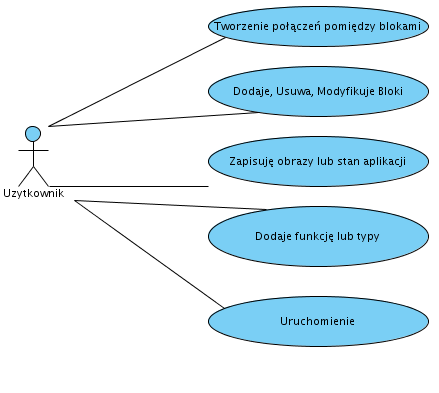
\includegraphics[scale=0.7]{UseCase}
\end{center}
\caption{Sposoby użycia}
\label{fig:usecase}
\end{figure}
\newpage 
\subsection{Struktura}
\subsubsection{Silnik aplikacji}
Diagram Przestawiający tylko i~wyłącznie silnik aplikacji, nie ma tutaj ujętego~GUI.
\\
Klasy:
\begin{enumerate}
\item Item - jeden z~elementów który będzie używany do opisu konfiguracji bloków, przechowuję informację o~najmniejszym ``atomie'' takie jak typ 
(np: bitmap,string,int,double), name (np: width, height, byte), oraz wartość. 
\item Block - klasa opisująca blok, zawiera jego konfigurację (BlockConfig), oraz jego wejścia i~wyjścia.
\item BlockConfig - Konfiguracja jednego bloku, w~obiekcie map zapisana jest lista obiektów. 
\item BlockElement - klasa reprezentująca wejscia/wyjscia miedzy blokami, zawiera - nazwę, opis, stan - czy jest poprawnie podłączony (errorCode) 
\item BlockInput - klasa opisująca tylko wejścia.
\item BlockOutput - klasa opisująca tylko wyjścia.
\item FunctionDll - klasa obsługująca nowe funkcję z~dll.
\item PluginContener - przechowuję listę typów i~funkcji z~dll.
\item TypeConfig - typ który będzie przesyłany do bloku.
\item TypeDll - klasa obsługująca nowe typy z~dll.
\end{enumerate}

\begin{figure}[htbp]
\begin{center}
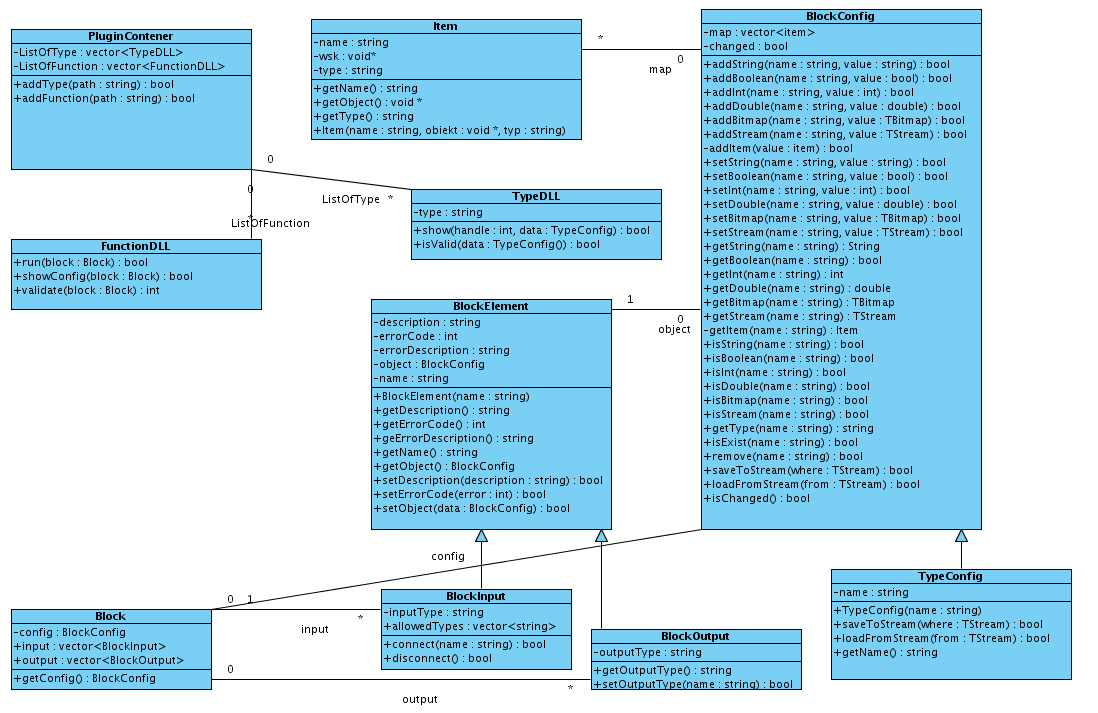
\includegraphics[angle=90,scale=0.5]{ClassDiagram}
\end{center}
\caption{Diagram Klas}
\label{fig:ClassDiagram}
\end{figure}
\newpage
\subsubsection{GUI}
\begin{figure}[h]
\begin{center}
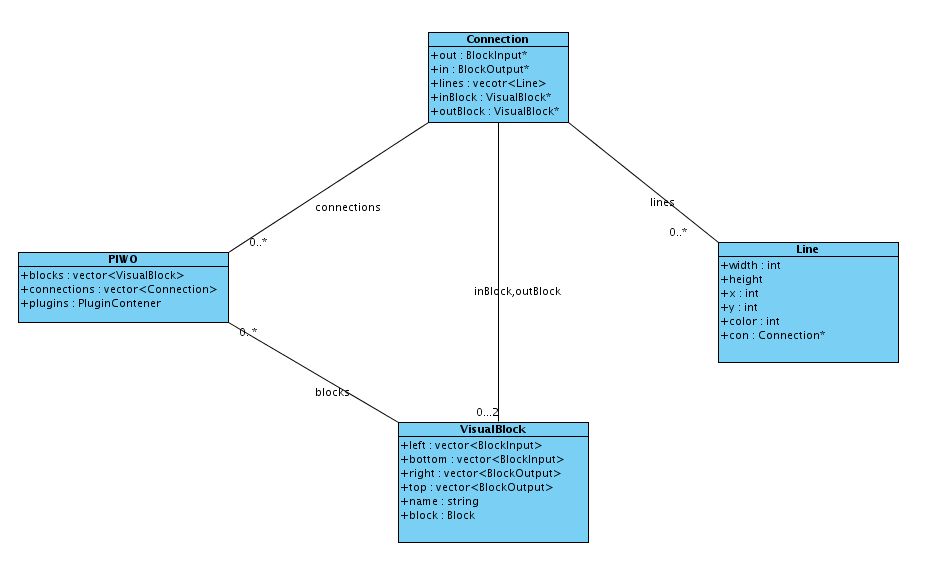
\includegraphics[scale=0.5]{ClassDiagram-GUI}
\end{center}
\caption{Diagram Klass dla Interfejsu Graficznego}
\label{fig:ClassDiagram-GUI}
\end{figure}
\subsection{Słownik systemu}

\section{Etap implementacji}
\subsection{Formatowanie Kodu}
Kod programu będzie tworzony z~myślą o~automatycznym tworzeniu dokumentacji przy użyciu doxygen. Poniżej przykład formatowania:
\begin{verbatim}
/**
 *  Przykładowa klasa. i jakis opis do niej. 
 *  @author Piotr Wilk
 *  @date 2008.11.19
 *  @version 1.0
 */

class Test
{
  public:
      
      /**
       *  Konstruktor.
       *  Opis konstruktora co robi itp.
       */
      Test();

      /**
       * Destruktor
       * Opis Destruktora
       */
     ~Test();
    
      /**
       * Opis funkcji.
       * @param a opis argumentu a
       * @param s opis argumentu s 
       * @see Test()
       * @see ~Test()
       * @see publicVar()
       * @return opis 
       */
       int testMe(int a,const char *s);
       
      /** 
       * a public variable.
       * Details.
       */
       int publicVar;
       
};
\end{verbatim}
\section{Etap “wdrożenia”}
\end{document}
